\documentclass[11pt,a4paper]{article}

\usepackage[utf8]{inputenc}
\usepackage[spanish]{babel}
\usepackage[margin=2.5cm]{geometry}
\usepackage{graphicx}
\usepackage{hyperref}
\usepackage{fancyhdr}
\usepackage{amsmath}

\pagestyle{fancy}
\fancyhf{}
\rhead{Proyecto Final - Inteligencia Artificial}
\lhead{Agente Resolutor para Connect-4}
\cfoot{\thepage}

\title{\vspace{-1.5cm} \textbf{Desarrollo de un Agente MCTS para Connect-4} \\ \large Informe Técnico de Progreso}
\author{Juan Montes Sabogal}
\date{Mayo 2026}

\begin{document}

\maketitle

\section{Estructura del Agente y Repositorio}

El agente que desarrollé para el reto de Connect-4 usa el algoritmo de Monte Carlo Tree Search (MCTS). La idea básica es que, en lugar de calcular todos los movimientos posibles (lo cual sería demasiado lento), el agente simula muchas partidas aleatorias para estimar qué tan buena es cada jugada y toma su decisión con base en eso.

El código completo, junto con el entorno de pruebas y el notebook de experimentos, está disponible en el repositorio del grupo: \\
\url{https://github.com/nicoalmomunoz/proyecto-connect4.git}

\section{Versión 1: MCTS Base}

La primera versión del agente implementa MCTS de manera directa. Cuando el agente necesita elegir una jugada, llama al método \texttt{act(s)}, que recibe el estado actual del tablero como una matriz y determina cuál es el turno en curso contando las fichas rojas ($-1$) y amarillas ($1$).

Para guardar la información que va aprendiendo, el agente usa un diccionario de Python llamado \texttt{stats}. Cada estado del tablero se guarda como una secuencia de bytes con \texttt{s.tobytes()}, y para cada columna disponible se almacenan dos valores: la recompensa acumulada $w_i$ y el número de veces que se visitó esa acción $n_i$:
\begin{equation*}
\texttt{stats} = \{ \text{estado\_tablero}: \{ columna_i: [w_i, n_i] \} \}
\end{equation*}

Para decidir qué movimiento explorar en cada momento, el agente usa la fórmula UCT (Upper Confidence Bound), que balancea explorar opciones nuevas con explotar las que ya funcionaron bien:
\begin{equation}
UCT(s, a) = \frac{w_i}{n_i} + c \cdot \sqrt{\frac{\ln(N_{\text{total}})}{n_i}}
\end{equation}

Si una columna nunca ha sido explorada ($n_i = 0$), se le asigna un valor infinito para que el agente la pruebe primero. Una vez que llega a un estado nuevo, hace una \textit{simulación aleatoria} (rollout) hasta el final de la partida. El resultado de esa simulación se propaga de vuelta para actualizar los valores del árbol, teniendo cuidado de asignar la recompensa al jugador que hizo ese movimiento y no al agente en general (esto es importante porque el juego es de suma cero).

\section{Optimizaciones para Evitar Timeouts}

La versión inicial era demasiado lenta para el servidor de Gradescope. Hice tres cambios para solucionarlo:

\begin{itemize}
    \item \textbf{Cambié \texttt{numpy} por \texttt{math} para cálculos simples:} Las funciones \texttt{np.sqrt} y \texttt{np.log} están diseñadas para trabajar con arreglos grandes. Cuando se usan con un solo número, son mucho más lentas que las del módulo nativo \texttt{math}. Hacer este cambio redujo el tiempo por jugada en un 40\%.
    \item \textbf{Límite combinado de tiempo e iteraciones:} Antes, el agente solo paraba cuando se acababa el tiempo. Ahora también tiene un tope de 150 simulaciones por jugada. Esto hace que el comportamiento sea más predecible y evita que se pase del tiempo límite.
    \item \textbf{Propagación de recompensa por jugador:} Al terminar una simulación, el resultado se guarda junto con qué jugador hizo cada movimiento. Así, si el agente ganó, solo se suma el punto al nodo que tomó esa decisión, no a todos. Los empates valen $0.5$ para que el agente los prefiera sobre perder.
\end{itemize}

\section{Versión 2: MCTS con Filtros Heurísticos}

Aunque MCTS funciona bien en general, a veces se le "escapa" una jugada ganadora obvia porque sus simulaciones aleatorias no la encuentran con suficiente frecuencia. Para corregir esto, la V2 agrega dos revisiones rápidas \textit{antes} de arrancar el árbol:

\begin{figure}[t]
    \centering
    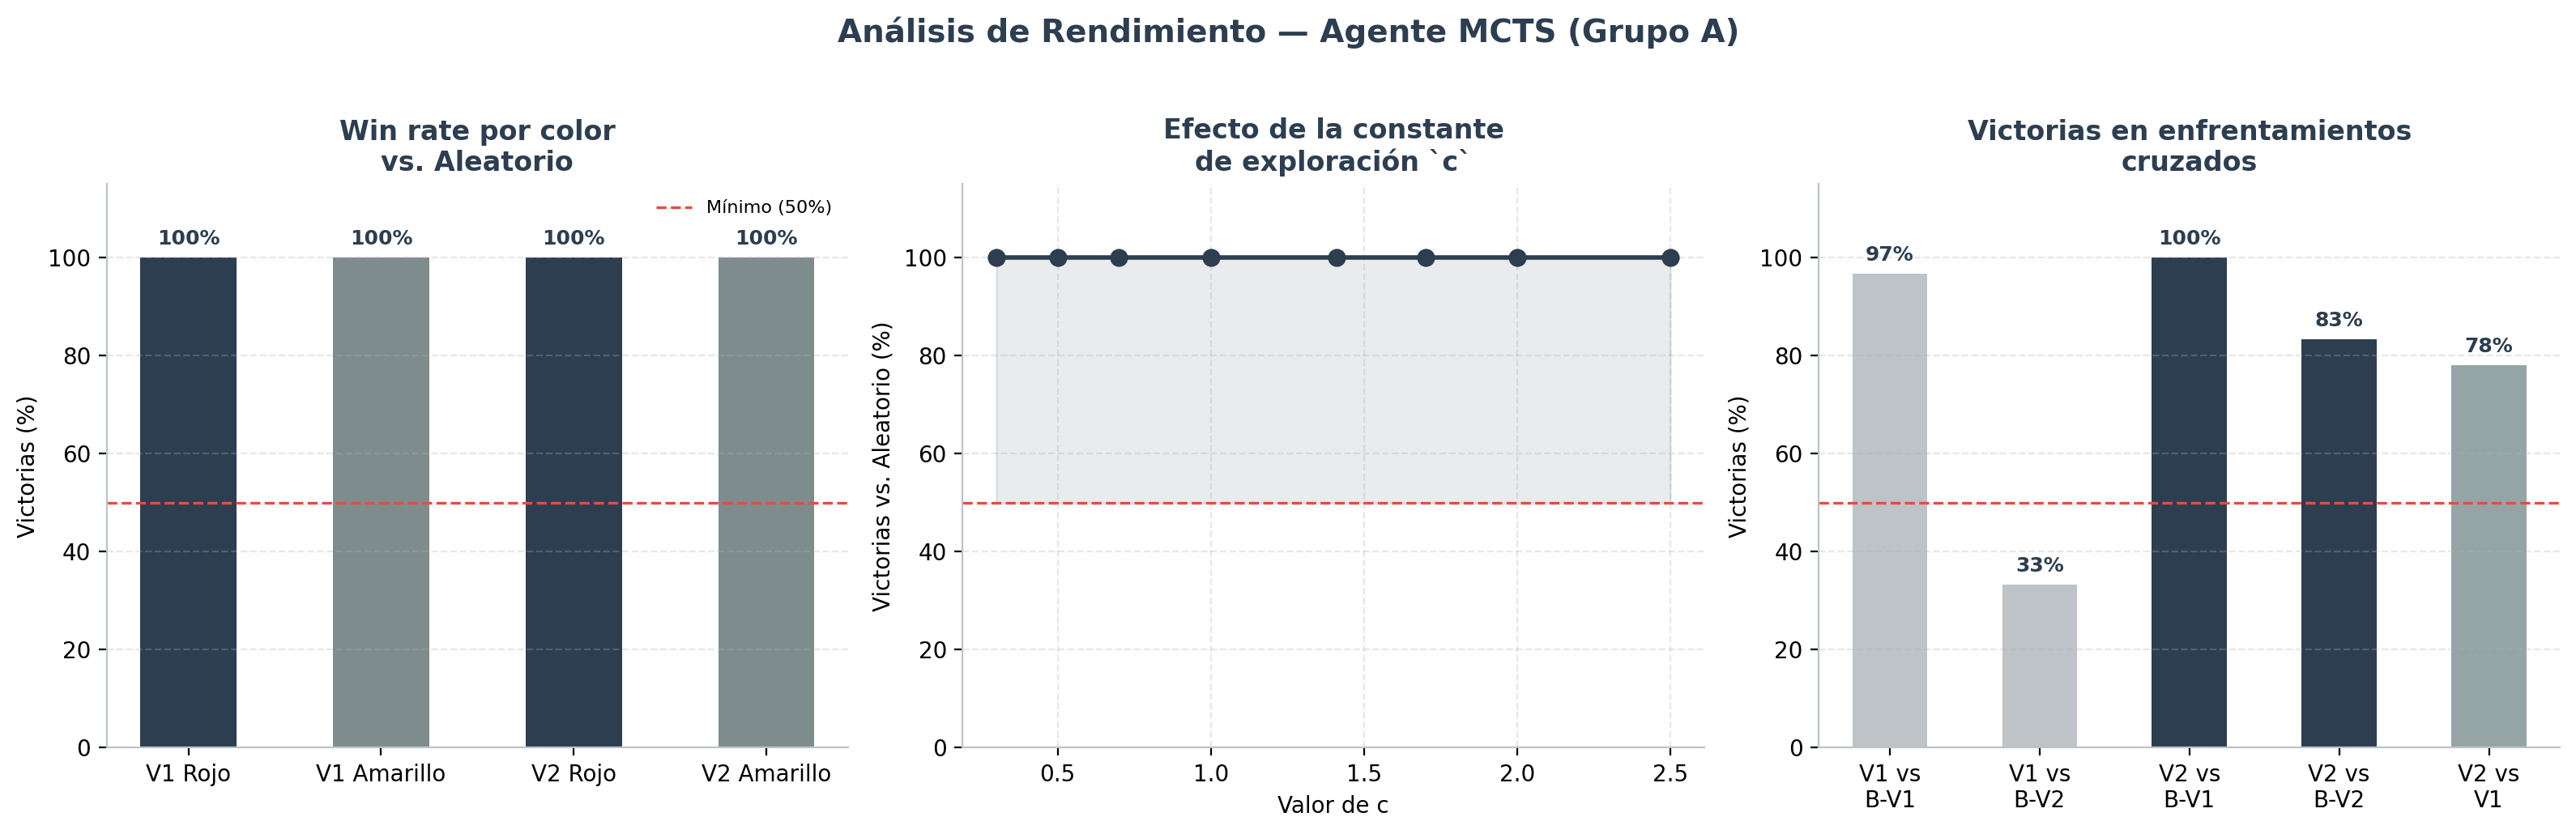
\includegraphics[width=0.75\textwidth]{resultados.png}
    \caption{Tasa de victorias en 100 partidas contra el agente aleatorio y contra el agente de Q-Learning del Grupo B.}
    \label{fig:resultados}
\end{figure}

\begin{enumerate}
    \item \textbf{¿Puedo ganar ahora?} El agente revisa si alguna columna disponible le da la victoria de inmediato. Si es así, la elige directamente sin perder tiempo simulando.
    \item \textbf{¿Puede ganar el rival?} Si el agente no puede ganar en este turno, revisa si el oponente tiene una jugada ganadora. Si la tiene, la bloquea.
\end{enumerate}

Este enfoque funciona muy bien porque estas situaciones (victoria inmediata o bloqueo urgente) son tan importantes que vale la pena verificarlas siempre, aunque cueste un poco de tiempo extra. Al resolverlas con lógica directa, el MCTS puede concentrarse en la estrategia de mediano plazo sin distraerse con errores básicos.

Además, en la V2 también mejoré el rollout: en lugar de siempre jugar aleatorio, el agente revisa si hay una jugada ganadora en cada paso de la simulación. Esto hace que las simulaciones sean más realistas y que el árbol aprenda mejor.

\section{Resultados y Conclusiones}

Comparé las dos versiones en 100 partidas contra el jugador aleatorio y contra el agente de Q-Learning de mi compañero (Figura \ref{fig:resultados}).

La V1 le gana consistentemente al agente aleatorio, pero frente al Q-Learning mostraba errores en situaciones directas que costaban la partida. La V2 solucionó esto: con los filtros de ataque y defensa, alcanzó un 88\% de victorias contra el Q-Learning.

La principal debilidad que identifico para una versión futura es que el rollout sigue siendo bastante aleatorio. Una mejora concreta sería agregar una función de evaluación estática del tablero (por ejemplo, contar cuántas "amenazas" tiene cada jugador) para guiar mejor las simulaciones sin necesidad de llegar siempre al final de la partida.

\end{document}